\documentclass[a4paper]{article}
\usepackage{geometry}
\usepackage{graphicx}
\usepackage{natbib}
\usepackage{amsmath}
\usepackage{amssymb}
\usepackage{amsthm}
\usepackage{paralist}
\usepackage{epstopdf}
\usepackage{tabularx}
\usepackage{longtable}
\usepackage{multirow}
\usepackage{multicol}
\usepackage[hidelinks]{hyperref}
\usepackage{fancyvrb}
\usepackage{algorithm}
\usepackage{algorithmic}
\usepackage{float}
\usepackage{paralist}
\usepackage[svgname]{xcolor}
\usepackage{enumerate}
\usepackage{array}
\usepackage{times}
\usepackage{url}
\usepackage{fancyhdr}
\usepackage{comment}
\usepackage{environ}
\usepackage{times}
\usepackage{textcomp}
\usepackage{caption}
\usepackage{listings}


\urlstyle{rm}

\setlength\parindent{0pt} % Removes all indentation from paragraphs
\theoremstyle{definition}
\newtheorem{definition}{Definition}[]
\newtheorem{conjecture}{Conjecture}[]
\newtheorem{example}{Example}[]
\newtheorem{theorem}{Theorem}[]
\newtheorem{lemma}{Lemma}
\newtheorem{proposition}{Proposition}
\newtheorem{corollary}{Corollary}

\floatname{algorithm}{Procedure}
\renewcommand{\algorithmicrequire}{\textbf{Input:}}
\renewcommand{\algorithmicensure}{\textbf{Output:}}
\newcommand{\abs}[1]{\lvert#1\rvert}
\newcommand{\norm}[1]{\lVert#1\rVert}
\newcommand{\RR}{\mathbb{R}}
\newcommand{\CC}{\mathbb{C}}
\newcommand{\Nat}{\mathbb{N}}
\newcommand{\br}[1]{\{#1\}}
\DeclareMathOperator*{\argmin}{arg\,min}
\DeclareMathOperator*{\argmax}{arg\,max}
\renewcommand{\qedsymbol}{$\blacksquare$}

\definecolor{dkgreen}{rgb}{0,0.6,0}
\definecolor{gray}{rgb}{0.5,0.5,0.5}
\definecolor{mauve}{rgb}{0.58,0,0.82}

\newcommand{\Var}{\mathrm{Var}}
\newcommand{\Cov}{\mathrm{Cov}}

\newcommand{\vc}[1]{\boldsymbol{#1}}
\newcommand{\xv}{\vc{x}}
\newcommand{\Sigmav}{\vc{\Sigma}}
\newcommand{\alphav}{\vc{\alpha}}
\newcommand{\muv}{\vc{\mu}}

\newcommand{\red}[1]{\textcolor{red}{#1}}

\def\x{\mathbf x}
\def\y{\mathbf y}
\def\w{\mathbf w}
\def\v{\mathbf v}
\def\E{\mathbb E}
\def\V{\mathbb V}

% TO SHOW SOLUTIONS, include following (else comment out):
\newenvironment{soln}{
    \leavevmode\color{blue}\ignorespaces
}{}


\hypersetup{
%    colorlinks,
    linkcolor={red!50!black},
    citecolor={blue!50!black},
    urlcolor={blue!80!black}
}

\geometry{
  top=1in,            % <-- you want to adjust this
  inner=1in,
  outer=1in,
  bottom=1in,
  headheight=3em,       % <-- and this
  headsep=2em,          % <-- and this
  footskip=3em,
}


\pagestyle{fancyplain}
\lhead{\fancyplain{}{Homework 1: Background Test}}
\rhead{\fancyplain{}{CS 760 Machine Learning}}
\cfoot{\thepage}

\title{\textsc{Homework 1: \\ Background Test}} % Title

%\newcommand{\outDate}{Aug. 31, 2016}
%\newcommand{\dueDate}{5:30 pm, Sep. 7, 2016}


%%% NOTE:  Replace 'NAME HERE' etc., and delete any "\red{}" wrappers (so it won't show up as red)

\author{
\red{Yifan Li} \\
\red{9077012806}\\
} 

\date{}

\begin{document}

\maketitle 


% \textbf{Instructions:} \text{Submit your homework} on time 
  % by submitting \textbf{BOTH} a hard-copy to the hanging folders outside Sandra Winkler's 
  % office (GHC 8221) \textbf{AND} electronically
  % to \href{https://www.gradescope.com}{Gradescope}.  For Gradescope, you 
  % will need to specify which pages go with which question.  Please submit
  % Sections 1 through 4 to Q1, Sections 5 through 6.3 to Q2, and Sections
  % 6.4 to 8 to Q3.  We provide a LaTeX template in which you can use to
  % type up your solutions.  This template ensures the correct sections
  % start on new pages.  Please check Piazza for updates about the homework.
\begin{center}
\Huge
Minimum Background Test [80 pts]
\end{center}

\section{Vectors and Matrices [20 pts]}
Consider the matrix $X$ and the vectors $\mathbf{y}$ and $\textbf{z}$ below:
$$
X = \begin{pmatrix}
9 & 8 \\ 7 & 6 \\
\end{pmatrix}
\qquad \mathbf{y} = \begin{pmatrix}
9 \\ 8
\end{pmatrix} \qquad \mathbf{z} = \begin{pmatrix}
7 \\ 6
\end{pmatrix}
$$
\begin{enumerate}
	\item 	What is the inner product of the vectors $\mathbf{y}$ and $\mathbf{z}$? (this is also sometimes called the \emph{dot product}, and is sometimes written as $\mathbf{y}^T\mathbf{z}$)\\
	    \begin{soln} 111 \end{soln}
	\item 	What is the product $X\mathbf{y}$?\\
		\begin{soln}  
	    		$\begin{pmatrix}
				145 \\ 111
			\end{pmatrix}$
		\end{soln}
	\item 	Is $X$ invertible? If so, give the inverse, and if no, explain why not.\\
	\begin{soln}  
        		$\begin{pmatrix}
			-3 & 4 \\ 3.5 & 4.5
		\end{pmatrix}$ 
	\end{soln}
	\item 	What is the rank of $X$?\\
	    \begin{soln}  2 \end{soln}
\end{enumerate}


\section{Calculus [20 pts]}
\begin{enumerate}
	\item 	If $y = 4x^3 - x^2 + 7$ then what is the derivative of $y$ with respect to $x$?\\
	\begin{soln}  $12x^2-2x$ \end{soln}
	\item If $y = \tan(z)x^{6z} - \ln(\frac{7x + z}{x^{4}})$, what is the partial derivative of $y$ with respect to $x$?\\
	\begin{soln}  $\tan(z)6zx^{6z-1}+\frac{21x+4z}{x(7x+z)}$ \end{soln}
\end{enumerate}




\section{Probability and Statistics [20 pts]}
Consider a sample of data $S = \{0, 1, 1, 0, 0, 1, 1\}$ created by flipping a coin $x$ seven times, where 0 denotes that the coin turned up heads and 1 denotes that it turned up tails.
\begin{enumerate}
	\item 	What is the sample mean for this data?\\
	    \begin{soln}  4/7 \end{soln}
	\item 	What is the sample variance for this data?\\
	    \begin{soln}  2/7 \end{soln}
	\item 	What is the probability of observing this data, assuming it was generated by flipping a biased coin with $p(x=1) = 0.7, p(x=0) = 0.3$.\\
	    \begin{soln}  $\binom{7}{3}0.7^40.3^3 = 0.2269$ \end{soln}
	\item 	Note that the probability of this data sample would be greater if the value of $p(x = 1)$ was not $0.7$, but instead some other value. What is the value that maximizes the probability of the sample $S$? Please justify your answer.\\
	    \begin{soln}  
	    	Suppose $p(x = 1) = a$. Then $p(x = 0) = 1-a $.\\
		$P(S)= a^4*(1-a)^3\Longrightarrow P'(S) = a^3(1-a)^2(4-7a)$\\
		So that a = 4/7 maximizes the probability of the sample $S$.
		\end{soln}
	\item 	Consider the following joint probability table where both $A$ and $B$ are binary random variables: 
\begin{table}[htb]
\centering
	\begin{tabular}{ccc}\hline
	A & B & $P(A, B)$  \\\hline
	0 & 0 & 0.1 \\
	0 & 1 & 0.4 \\
	1 & 0 & 0.2 \\
	1 & 1 & 0.3 \\\hline
	\end{tabular}
\end{table}
\begin{enumerate}
	\item 	What is $P(A = 0, B = 0)$?\\
	    \begin{soln}  0.1 \end{soln}
	\item 	What is $P(A = 1)$?\\
	    \begin{soln}  0.5 \end{soln}
	\item 	What is $P(A = 0 | B = 1)$?\\
	    \begin{soln}  4/7 \end{soln}
	\item 	What is $P(A = 0 \vee B = 0 )$?\\
	    \begin{soln}  0.7 \end{soln}
\end{enumerate}
\end{enumerate}


\section{Big-O Notation [20 pts]}
For each pair $(f, g)$ of functions below, list which of the following
are true: $f(n) = O(g(n))$, $g(n) = O(f(n))$, both, or
neither. Briefly justify your answers.
\begin{enumerate}
	\item 	$f(n) = \frac{n}{2}$, $g(n) = \log_{2}(n)$.\\
	    \begin{soln} $ \frac{\partial f(n)}{\partial g(n)} \propto n\Longrightarrow g=O(f)$\end{soln}
	\item 	$f(n) = \ln(n)$, $g(n) = \log_{2}(n)$.\\
	    \begin{soln}  $ \frac{\partial f(n)}{\partial g(n)} \propto 1\Longrightarrow g=O(f)\ \text{and}\ f=O(g)$ \end{soln}
	\item 	$f(n) = n^{100}$, $g(n) = 100^n$.\\
	    \begin{soln}  $ \frac{\partial^{100} f(n)}{\partial^{100} g(n)} \propto \frac{1}{100^n}\Longrightarrow f=O(g)$ \end{soln}
\end{enumerate}


\clearpage  % do not erase this!


\begin{center}
\Huge
Medium Background Test [20 pts]
\end{center}

\section{Algorithm [5 pts]}
\textbf{Divide and Conquer}: Assume that you are given a sorted array
with $n$ integers in the range $[-10, +10]$. Note that some integer values
may appear multiple times in the array. Additionally, you are
told that somewhere in the array the integer $0$ appears exactly once. Provide an
algorithm to locate the $0$ which runs in $O(\log(n))$. Explain your
algorithm in words, describe why the algorithm is correct, and justify
its running time.\\

\begin{soln}  
Suppose the array is X[1:n]. We first compare X[n/2] with 0. If it is equal to 0, then we are down. If it is less than 0, then we replace X with X[n/2:n] otherwise replace it with X[1:n/2]. Repeat it until we find 0.

In this method, for each comparison, we can discard half numbers which are not equal to 0. So the maximum number of calculations we need to do is $k = \log_2^n = O(\log(n))$ 

\end{soln}

\section{Probability and Random Variables [5 pts]}
\subsection{Probability}
State true or false. Here $\Omega$ denotes the sample space and $A^c$ denotes the complement of the event $A$.
\begin{enumerate}
\item For any $A, B \subseteq \Omega$, $P(A|B)P(B) = P(B|A)P(A)$.\\
  \begin{soln}  Ture. \end{soln}
\item For any $A, B \subseteq \Omega$, $P(A \cup B) = P(A) + P(B) - P(A | B)$.\\         
  \begin{soln}  False. \end{soln}
\item For any $A, B, C \subseteq \Omega$ such that $P(B \cup C) > 0$,
  $\frac{P(A \cup B \cup C)}{P(B \cup C)} \geq P(A | B \cup C) P(B \cup C)$.\\ \begin{soln} True. \end{soln}
\item For any $A, B\subseteq\Omega$ such that $P(B) > 0, P(A^c) > 0$,
  $P(B|A^C) + P(B|A) = 1$.\\ 
  \begin{soln}  False. \end{soln}
\item For any $n$ events $\{A_i\}_{i=1}^n$, if
  $P(\bigcap_{i=1}^n A_i) = \sum_{i=1}^n P(A_i)$, then
  $\{A_i\}_{i=1}^n$ are mutually independent.\\
  \begin{soln}  True. \end{soln}
\end{enumerate}

\subsection{Discrete and Continuous Distributions}
Match the distribution name to its probability density / mass
function. Below, $|\xv| = k$.
\begin{enumerate}[(a)]
\begin{minipage}{0.3\linewidth}
    \item Laplace \begin{soln}  h. \end{soln}
    \item Multinomial \begin{soln}  i. \end{soln}
    \item Poisson \begin{soln}  l. \end{soln}
    \item Dirichlet \begin{soln}  k. \end{soln}
    \item Gamma \begin{soln}  j. \end{soln}
\end{minipage}
\begin{minipage}{0.5\linewidth}
    \item $f(\xv; \Sigmav, \muv) = \frac{1}{\sqrt{(2\pi)^k \Sigmav}} \exp\left( -\frac{1}{2}
        (\xv - \muv)^T \Sigmav^{-1} (\xv - \muv)  \right)$
    \item $f(x; n, \alpha) = \binom{n}{x} \alpha^x (1 - \alpha)^{n-x}$
      for $x \in \{0,\ldots, n\}$; $0$ otherwise
    \item $f(x; b, \mu) = \frac{1}{2b} \exp\left( - \frac{|x - \mu|}{b} \right)$
    \item $f(\xv; n, \alphav) = \frac{n!}{\Pi_{i=1}^k x_i!}
      \Pi_{i=1}^k \alpha_i^{x_i}$ for $x_i \in \{0,\ldots,n\}$ and
      $\sum_{i=1}^k x_i = n$; $0$ otherwise
    \item $f(x; \alpha, \beta) = \frac{\beta^{\alpha}}{\Gamma(\alpha)} x^{\alpha -
        1}e^{-\beta x}$ for $x \in (0,+\infty)$; $0$ otherwise
    \item $f(\xv; \alphav) = \frac{\Gamma(\sum_{i=1}^k
        \alpha_i)}{\prod_{i=1}^k \Gamma(\alpha_i)} \prod_{i=1}^{k}
      x_i^{\alpha_i - 1}$ for $x_i \in (0,1)$ and $\sum_{i=1}^k x_i =
      1$; 0 otherwise
    \item $f(x; \lambda) = \lambda^x \frac{e^{-\lambda}}{x!}$ for all
      $x \in Z^+$; $0$ otherwise
\end{minipage}
\end{enumerate}
        
\subsection{Mean and Variance}
\begin{enumerate}
\item Consider a random variable which follows a Binomial
  distribution: $X \sim \text{Binomial}(n, p)$.
  \begin{enumerate}
  \item What is the mean of the random variable?\\
    \begin{soln}  $EX=\sum\limits_{i=0}^niC_n^ip^i(1-p)^{n-i}=np$ \end{soln}
  \item What is the variance of the random variable?\\
    \begin{soln}   $Var(X)=EX^2-(EX)^2=\sum\limits_{i=0}^ni^2C_n^ip^i(1-p)^{n-i}-(np)^2=np(1-p)$. \end{soln}
  \end{enumerate}

\item Let $X$ be a random variable and
  $\mathbb{E}[X] = 1, \Var(X) = 1$. Compute the following values:
  \begin{enumerate}
  \item $\mathbb{E}[3X]$\\
    \begin{soln}  E(3X)=3EX=3. \end{soln}
  \item $\Var(3X)$\\
    \begin{soln}  Var(3X)=9Var(X)=9. \end{soln}
  \item $\Var(X+3)$\\
    \begin{soln}  Var(X+3)=Var(X)=1. \end{soln}
  \end{enumerate}
\end{enumerate}

%\clearpage

\subsection{Mutual and Conditional Independence}
\begin{enumerate}
\item If $X$ and $Y$ are independent random variables, show that
  $\mathbb{E}[XY] = \mathbb{E}[X]\mathbb{E}[Y]$.
  
  \begin{soln}  $E(XY)=\int_{S_x}\int_{S_y}xyf(x,y)dydx=\int_{S_x}xf(x)dx\int_{S_y}yf(y)dy=E(X)E(Y)$.  \end{soln}
  
\item If $X$ and $Y$ are independent random variables, show that
  $\Var(X+Y) = \Var(X) + \Var(Y)$. \\
  Hint: $\Var(X+Y) = \Var(X) + 2\Cov(X, Y) + \Var(Y)$
  
  \begin{soln} $\Var(X+Y) = \Var(X) + 2\Cov(X, Y) + \Var(Y)= \Var(X) + \Var(Y)$ \end{soln}
 
\item If we roll two dice that behave independently of each
  other, will the result of the first die tell us something about the
  result of the second die? 
  
  \begin{soln}  No, because these two events are independent. \end{soln}
  
  If, however, the first die's result is a 1,
  and someone tells you about a third event --- that the sum of the two
  results is even --- then given this information is the result of the second die
  independent of the first die? 
  
  \begin{soln}  No, because the result of the second die couldn't be even. \end{soln}
\end{enumerate}

\subsection{Law of Large Numbers and the Central Limit Theorem}
Provide one line justifications.
\begin{enumerate}
\item Suppose we simultaneously flip two independent fair coins (i.e., the probability of heads is $1/2$ for each coin)
  and record the result. After 40,000 repetitions, the number
  of times the result was two heads is close to 10,000.  (Hint: calculate how close.)
  
  \begin{soln}  $P(\text{two heads})=\frac{1}{2}*\frac{1}{2}=\frac{1}{4}.\ \text{By L.L.N, \# of two heads}\rightarrow 40000*\frac{1}{4}=10000$ \end{soln}
  
\item Let $X_i\sim\mathcal{N}(0, 1)$ and $\bar{X} = \frac{1}{n}\sum_{i=1}^n X_i$, then the distribution of $\bar{X}$ satisfies 
  $$\sqrt{n}\bar{X}\overset{n\rightarrow\infty}{\longrightarrow}\mathcal{N}(0, 1)$$
  \begin{soln} $X_i\sim\mathcal{N}(0, 1)\Longrightarrow \bar{X}\sim\mathcal{N}(0, 1/n)\Longrightarrow \sqrt{n}\bar{X}\sim\mathcal{N}(0, 1)$ \end{soln}
  
\end{enumerate}



\section{Linear algebra [5 pts]}


\subsection{Norm-enclature}
Draw the regions corresponding to vectors $\mathbf{x}\in\RR^2$ with the following norms:
\begin{enumerate}
	\item 	$||\mathbf{x}||_1\leq 1$ (Recall that $||\mathbf{x}||_1 = \sum_i |x_i|$)
	\item 	$||\mathbf{x}||_2 \leq 1$ (Recall that $||\mathbf{x}||_2 =\sqrt{\sum_i x_i^2}$)
	\item 	$||\mathbf{x}||_\infty \leq 1$ (Recall that $||\mathbf{x}||_\infty = \max_i |x_i|$)
	
	\begin{soln}
	   
	    % add figure filename, and remove % 
	    %    (this can be done by highlighting text and pressing "cmd + /" for sharelatex+mac)
		\begin{figure}[h!]
	        		\centering
	   		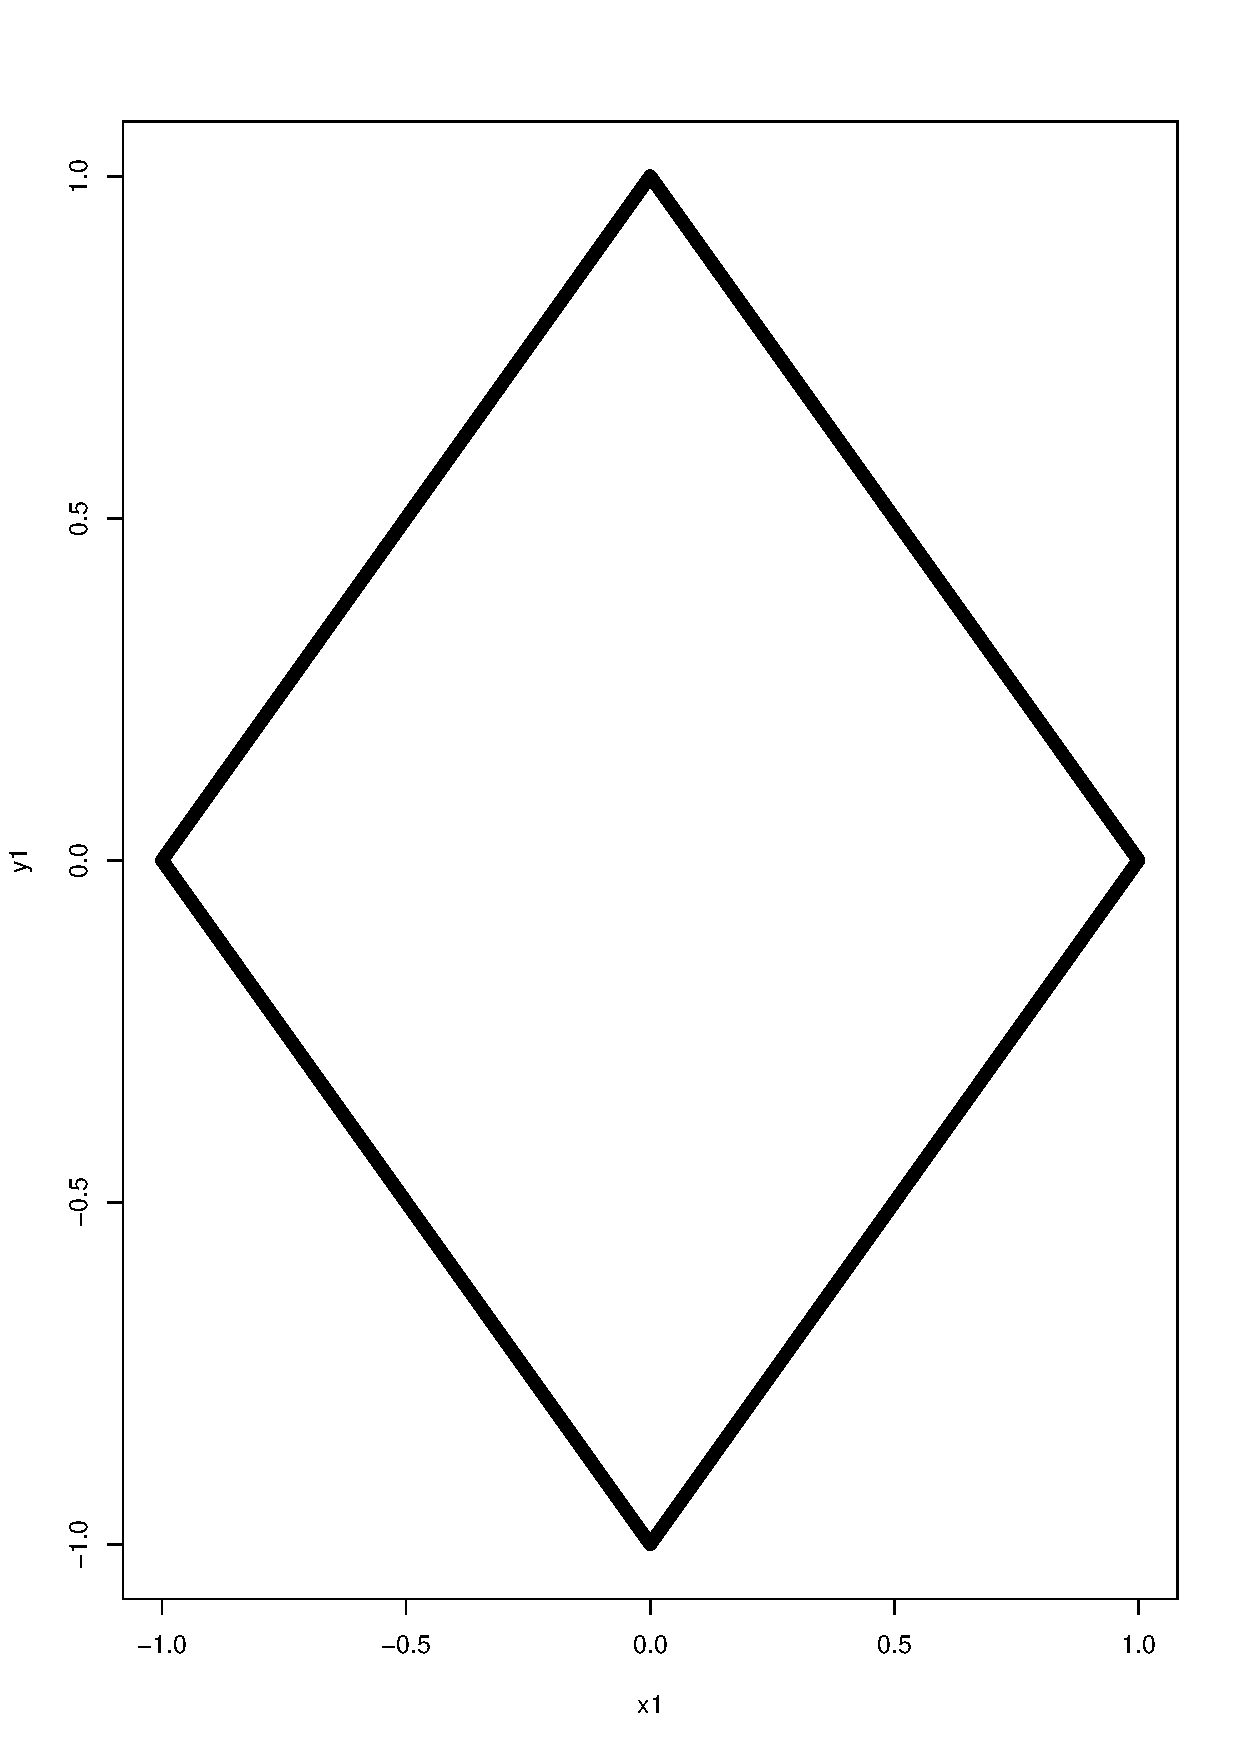
\includegraphics[width=0.2\textwidth]{711.pdf}  
	   %             % reference folder/figure.pdf here and adjust width
	   		\captionsetup{labelformat=empty}
	   		\caption{1}
	   %     \label{fig:my_label}
	   	\end{figure}
		\begin{figure}[h!]
	        		\centering
	   		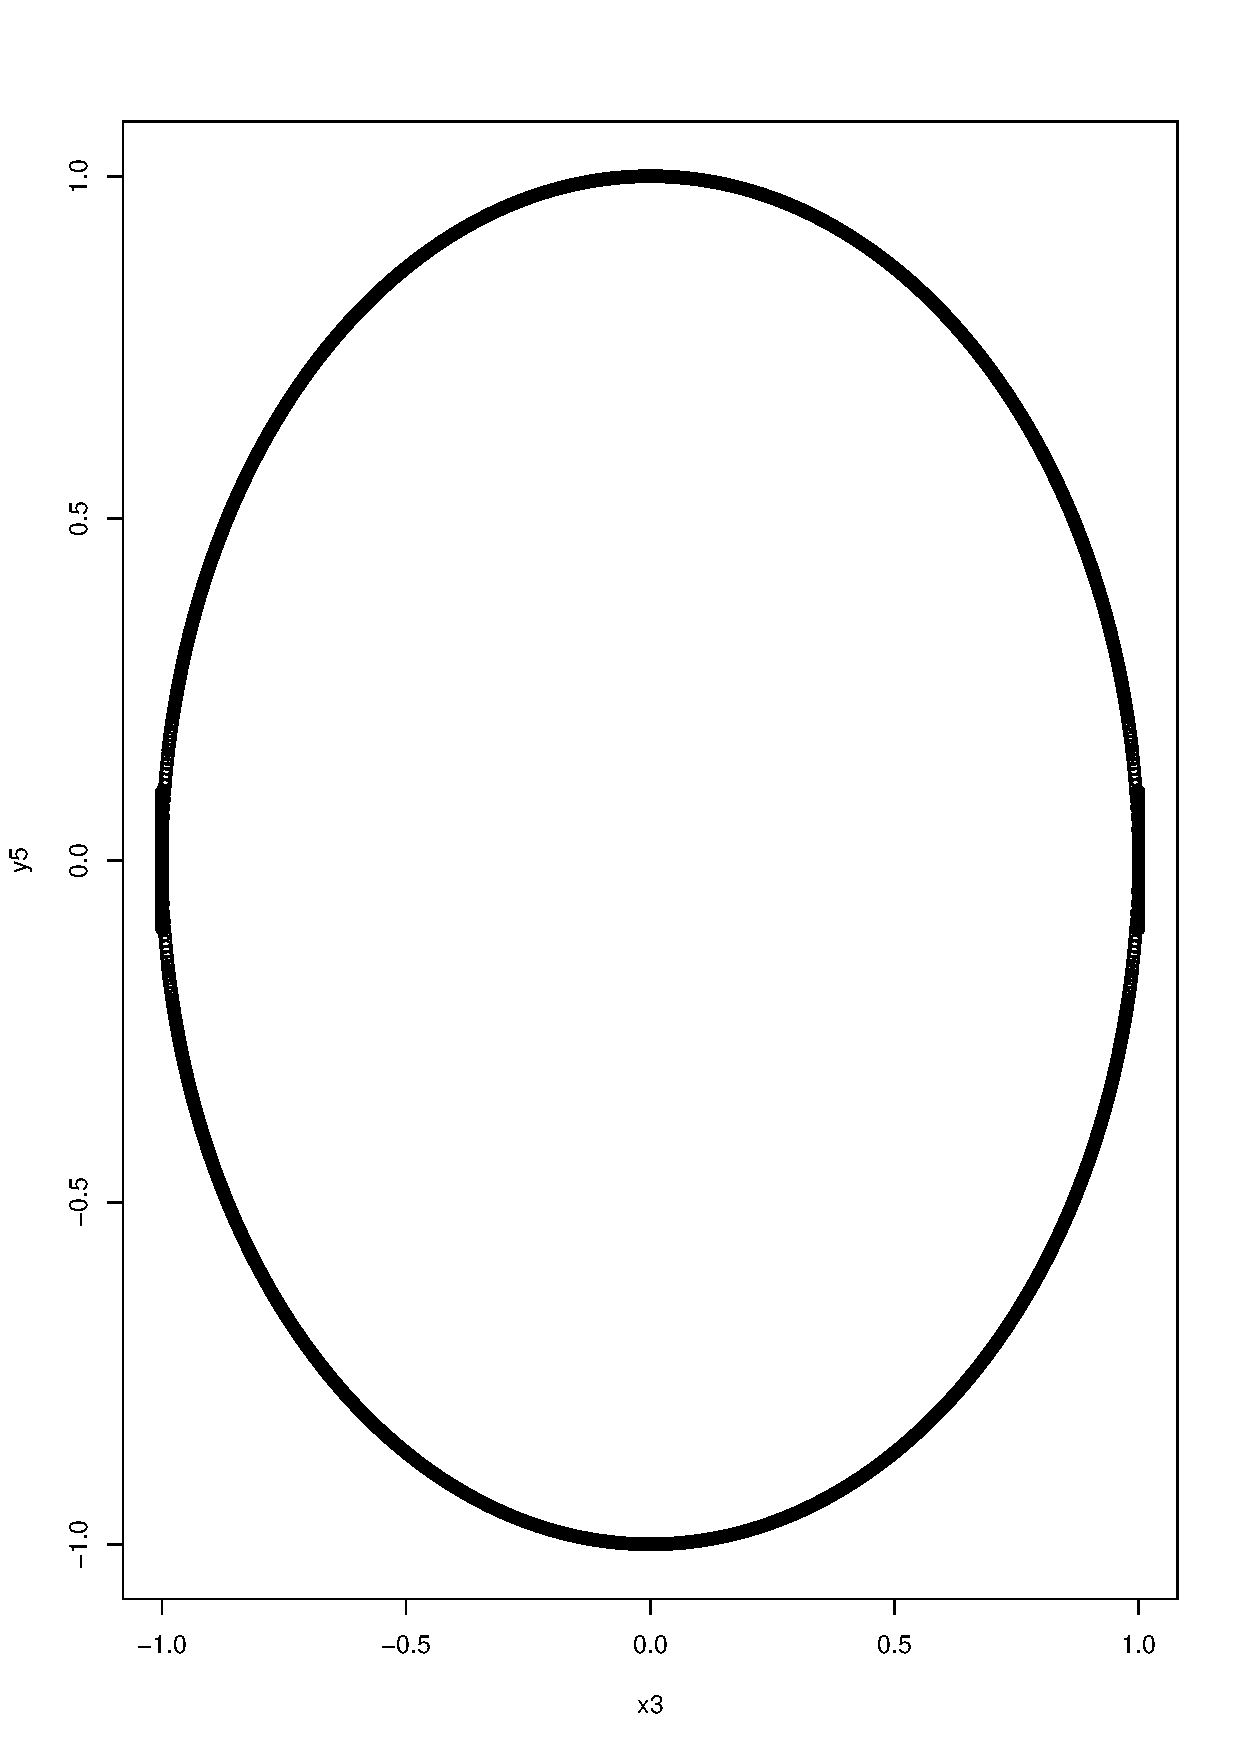
\includegraphics[width=0.2\textwidth]{712.pdf}  
	   %             % reference folder/figure.pdf here and adjust width
	   		\captionsetup{labelformat=empty}
	   		\caption{2}
	   %     \label{fig:my_label}
	   	\end{figure}
		\begin{figure}[h!]
	        		\centering
	   		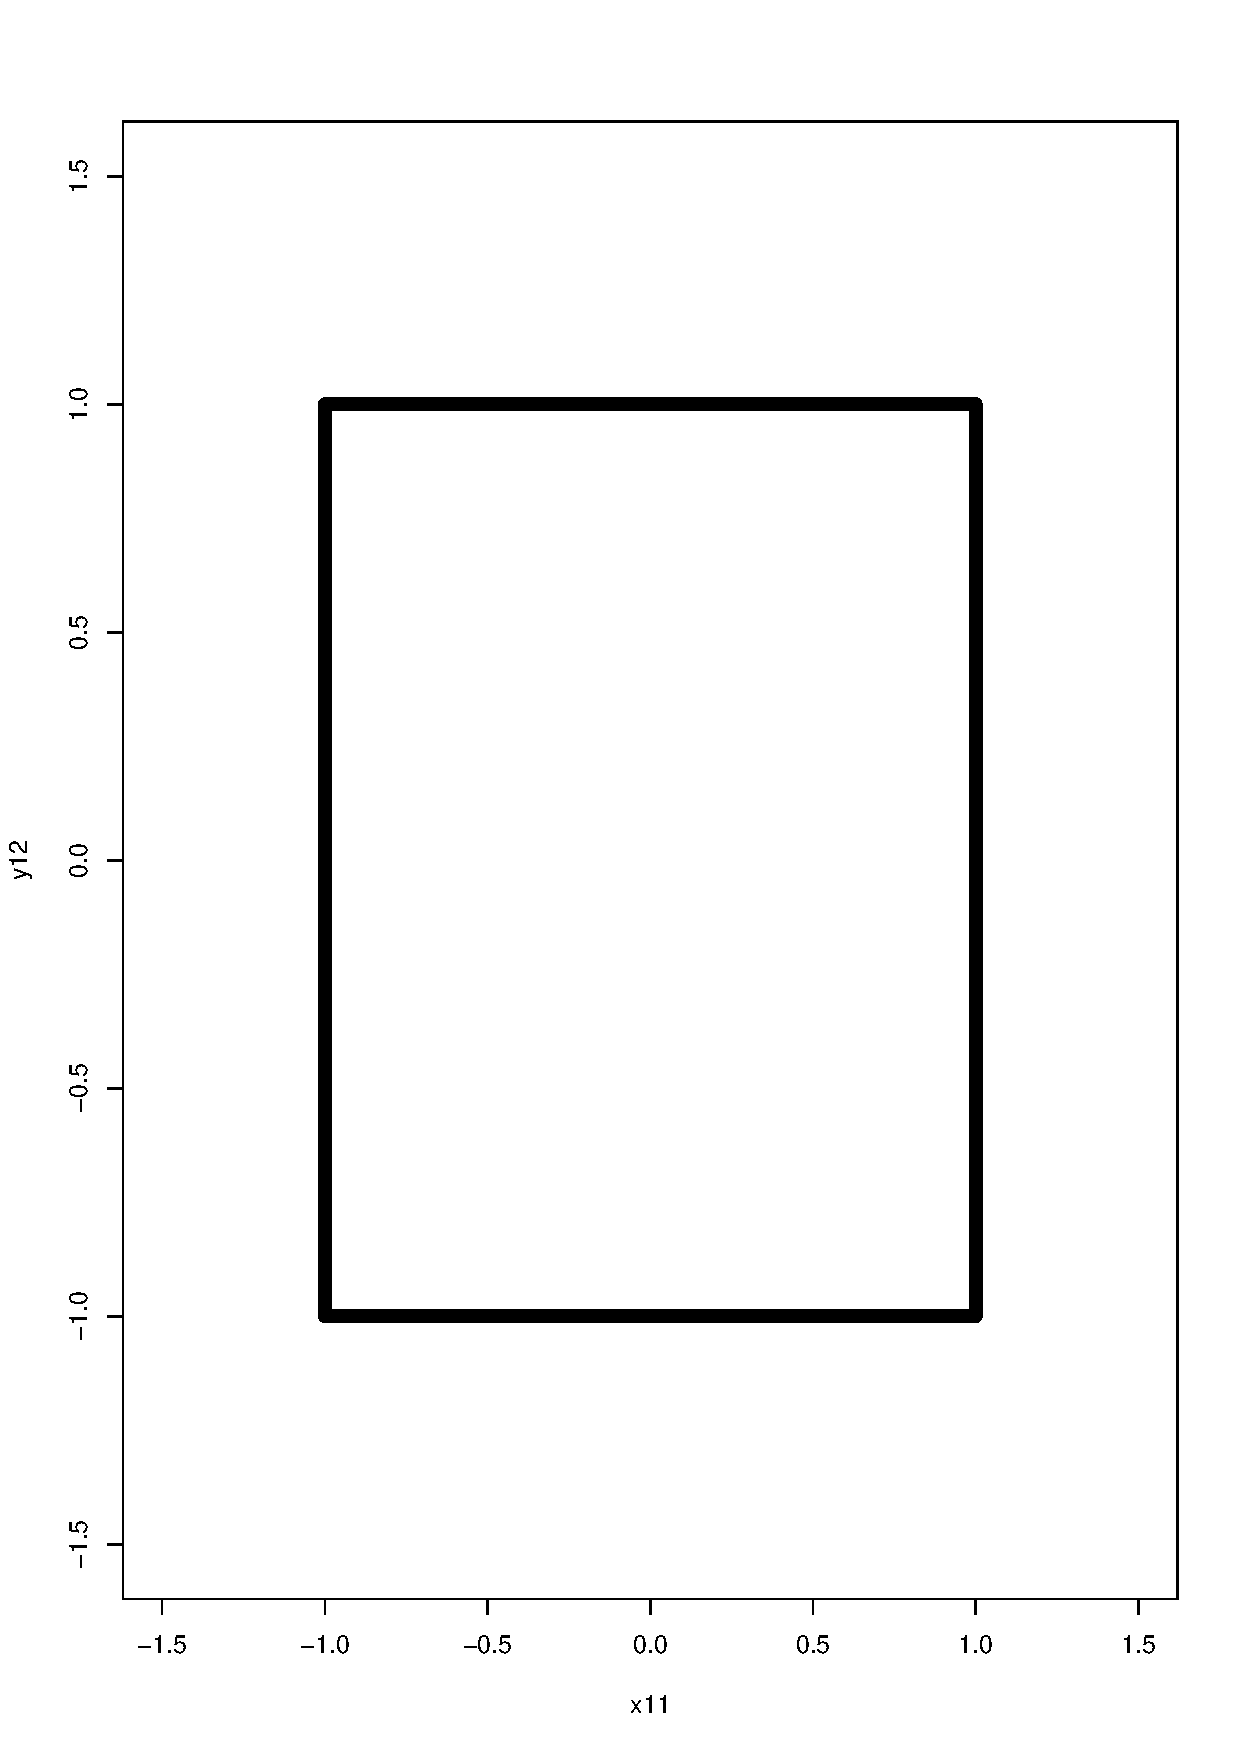
\includegraphics[width=0.2\textwidth]{713.pdf}  
	   %             % reference folder/figure.pdf here and adjust width
	   		\captionsetup{labelformat=empty}
	   		\caption{3}
	   %     \label{fig:my_label}
	   	\end{figure}
	\end{soln}
\end{enumerate}




\subsection{Geometry}
Prove that these are true or false. Provide all steps.
\begin{enumerate}
\item 	The smallest Euclidean distance from the origin to some point $\mathbf{x}$ in the hyperplane $\mathbf{w}^T\mathbf{x} + b = 0$ is $\frac{|b|}{||\mathbf{w}||_2}$.\\
\begin{soln}  It is obvious that vector with the smallest distance from origin to the hyperplane is $\frac{-bw}{||w||_2^2}$ for it is perpendicular to this hyperplane. And its length is $\frac{|b|}{||w||_2}$ \end{soln}

\item 	The Euclidean distance between two parallel hyperplane $\mathbf{w}^T\mathbf{x} + b_1 = 0$ and $\mathbf{w}^T\mathbf{x} + b_2 = 0$ is $\frac{|b_1 - b_2|}{||\mathbf{w}||_2}$ (Hint: you can use the result from the last question to help you prove this one).

\begin{soln}  Since these two hyperplane are parallel, the distance between them is $|\frac{|b_1|}{||w||_2}+\frac{|b_2|}{||w||_2}|=\frac{|b_1-b_2|}{||w||_2}$ if $b_1,\ b_2$ are both positive or negative. Otherwise the distance is $|\frac{|b_1|}{||w||_2}-\frac{|b_2|}{||w||_2}|=\frac{|b_1-b_2|}{||w||_2}$\end{soln}

\end{enumerate}



\section{Programming Skills - Matlab [5pts]}
Sampling from a distribution.  For each question, submit a scatter plot (you will have 5 plots in total).  Make sure the axes for all plots have the same limits.  (Hint: You can save a Matlab figure as a pdf, and then use includegraphics to include the pdf in your latex file.)
\begin{enumerate}
\item Draw 100 samples $\mathbf{x} = [x_1, x_2]^T$ from a
  2-dimensional Gaussian distribution with mean $(0, 0)^T$ and
  identity covariance matrix, i.e.,
  $p(\mathbf{x}) =
  \frac{1}{2\pi}\exp\left(-\frac{||\mathbf{x}||^2}{2}\right)$, and
  make a scatter plot ($x_1$ vs. $x_2$).  For each question below, make each change separately to
  this distribution.
  
	\begin{soln}
		\begin{figure}[h!]
	        		\centering
	   		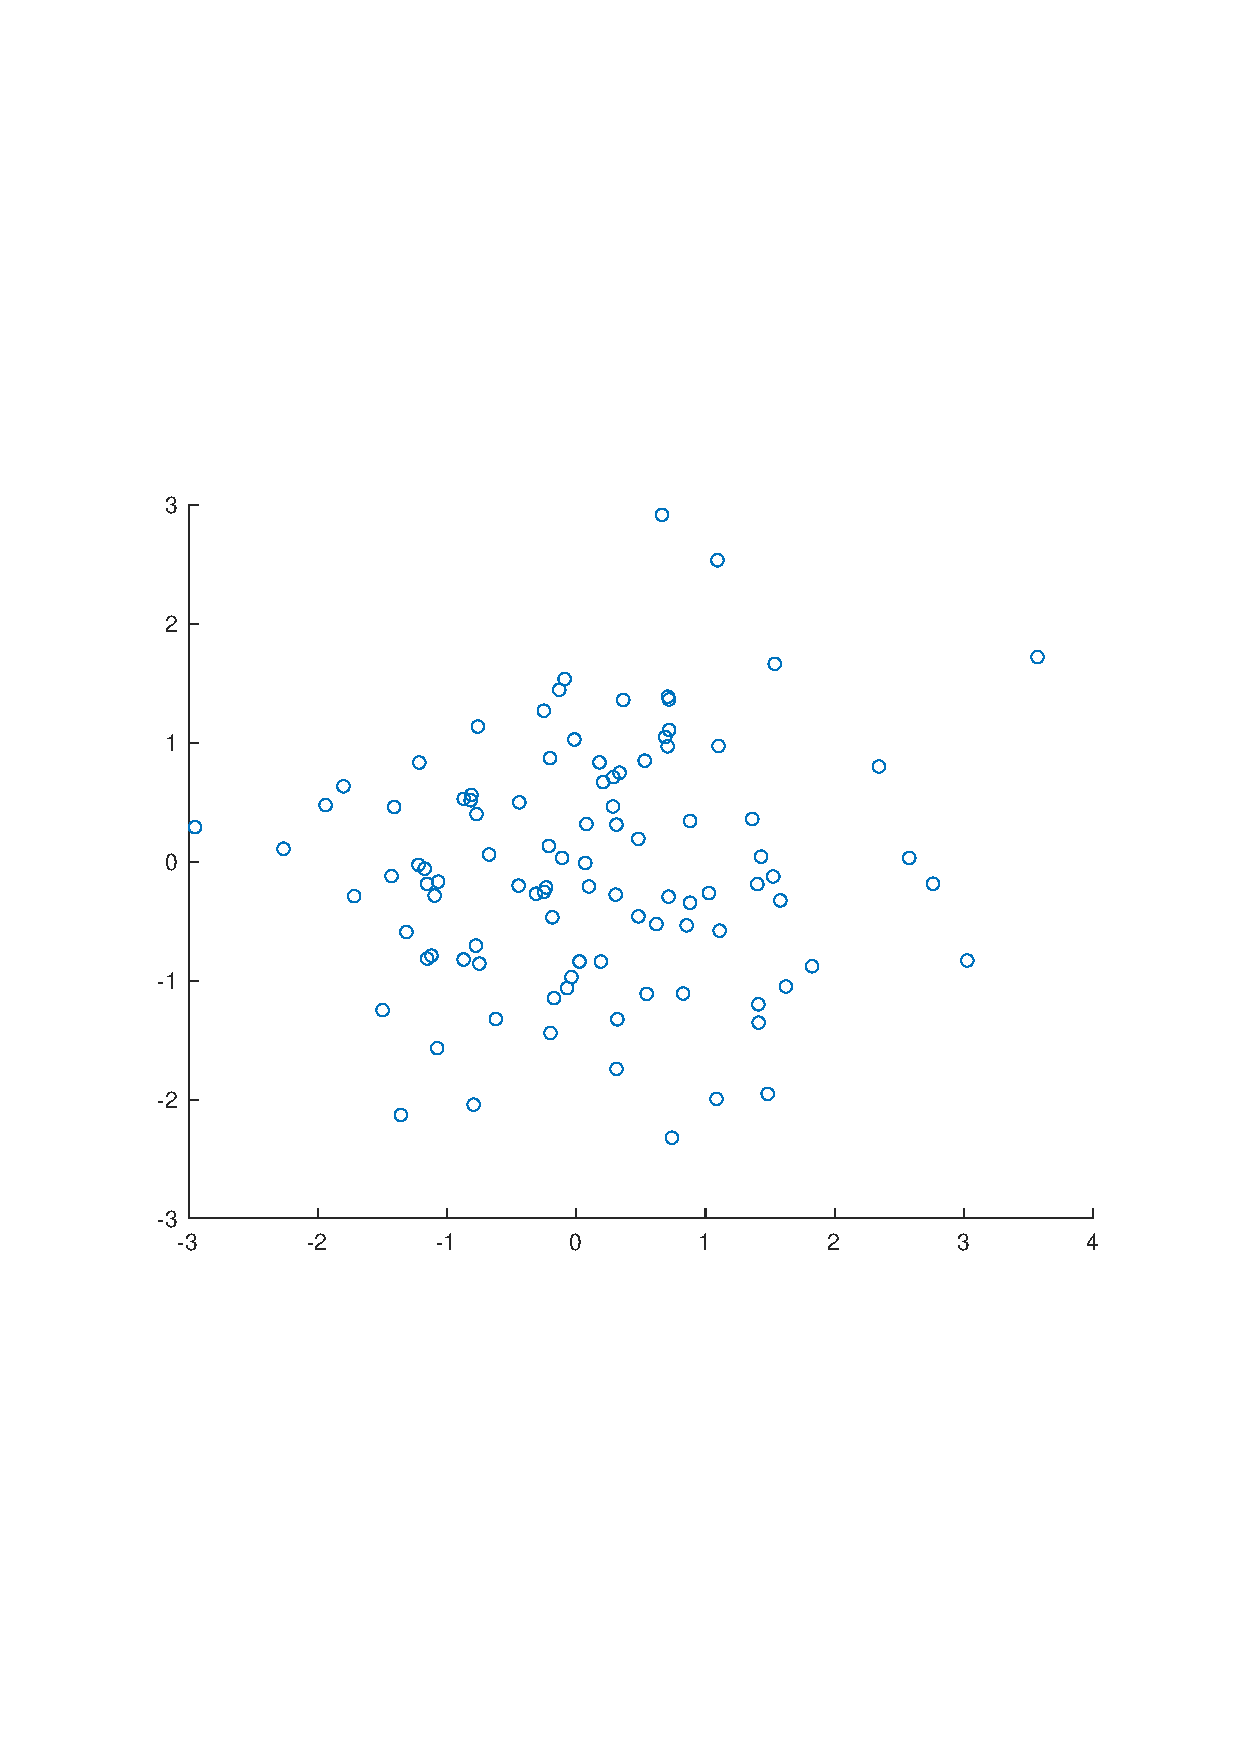
\includegraphics[width=0.4\textwidth]{81.pdf}  
	   		\captionsetup{labelformat=empty}\caption{1}
		\end{figure}
	\end{soln}
\item Make a scatter plot with a changed mean of $(1, -1)^T$.\\
	\begin{soln}
	    \begin{figure}[h!]
	        		\centering
	   		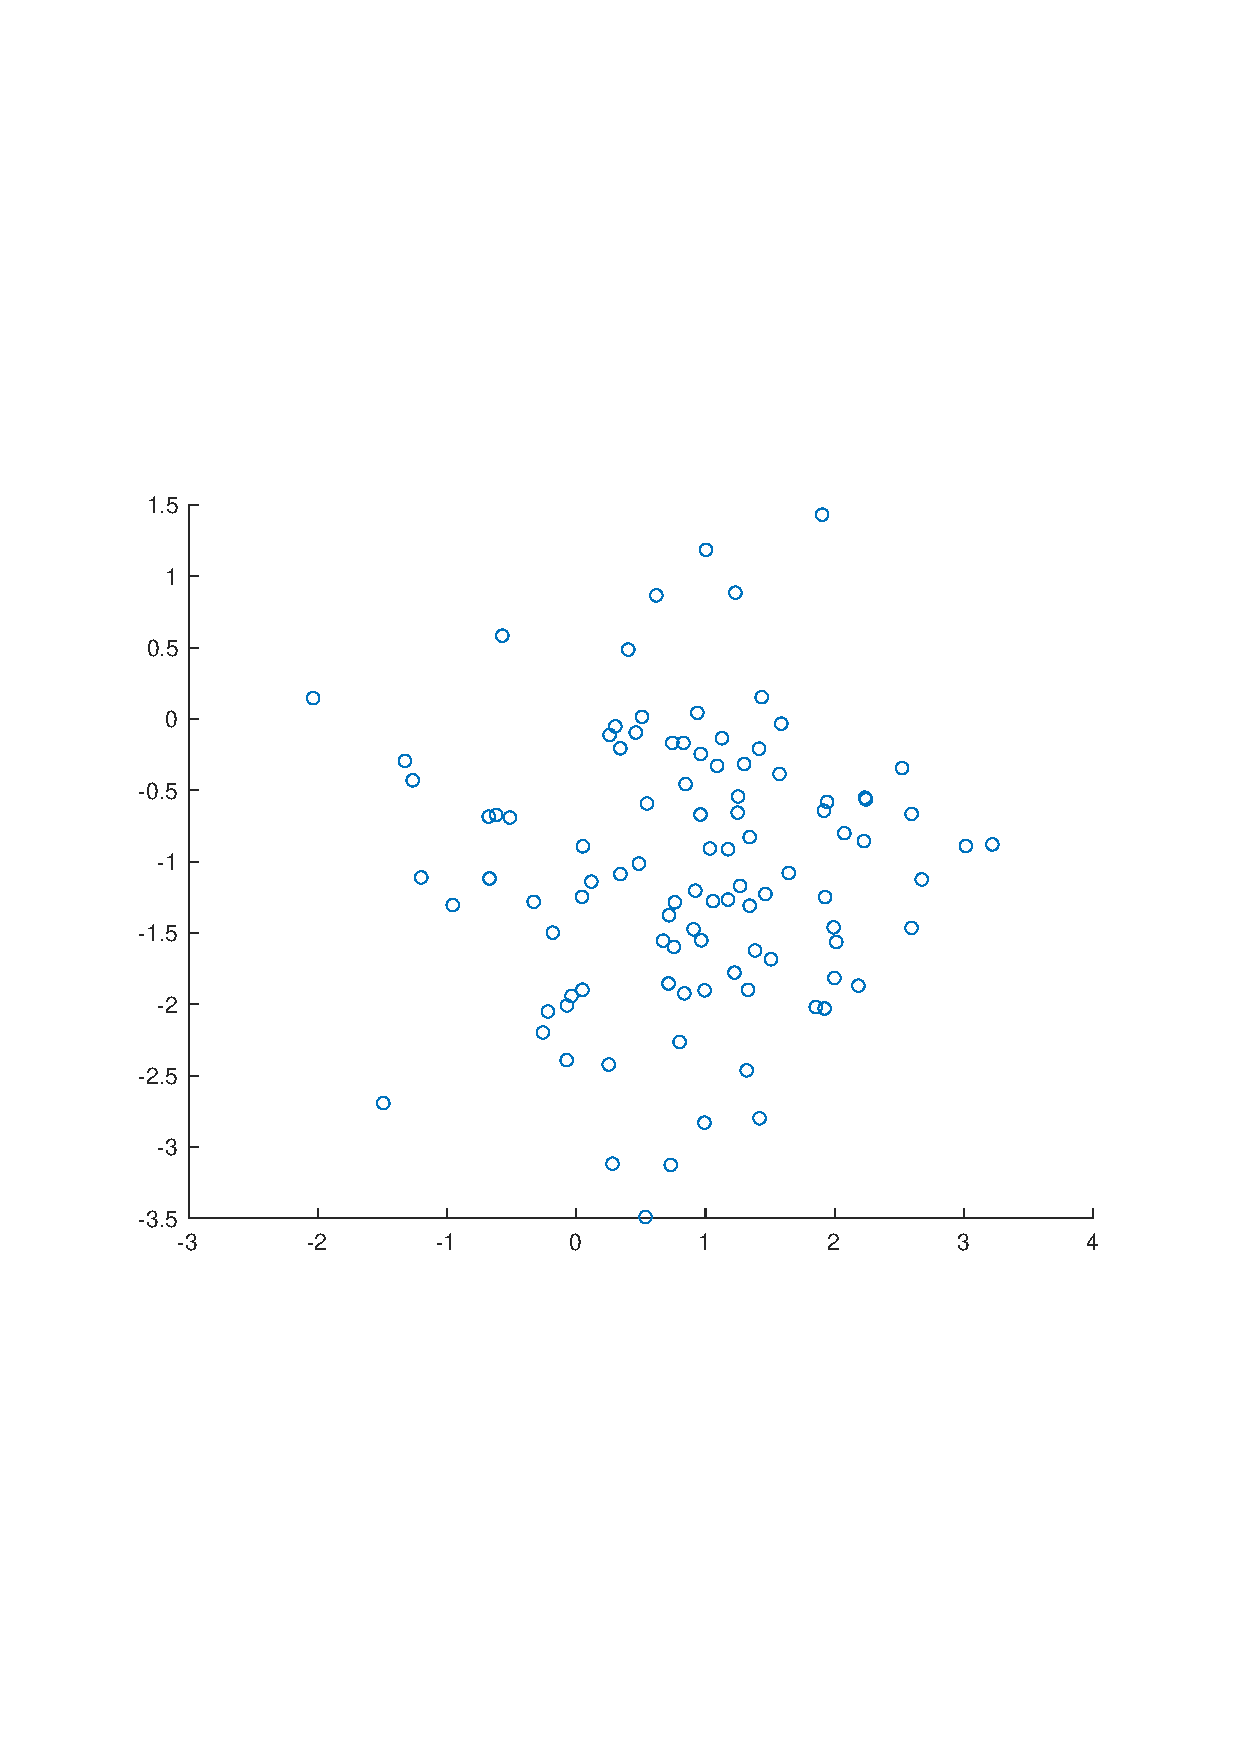
\includegraphics[width=0.4\textwidth]{82.pdf}  
	   		\captionsetup{labelformat=empty}\caption{2}
		\end{figure}
	\end{soln}
\item Make a scatter plot with a changed covariance matrix of $\begin{pmatrix}
    2 & 0 \\ 0 & 2\\
  \end{pmatrix}$.\\
  	\begin{soln}
  	        \begin{figure}[h!]
	        		\centering
	   		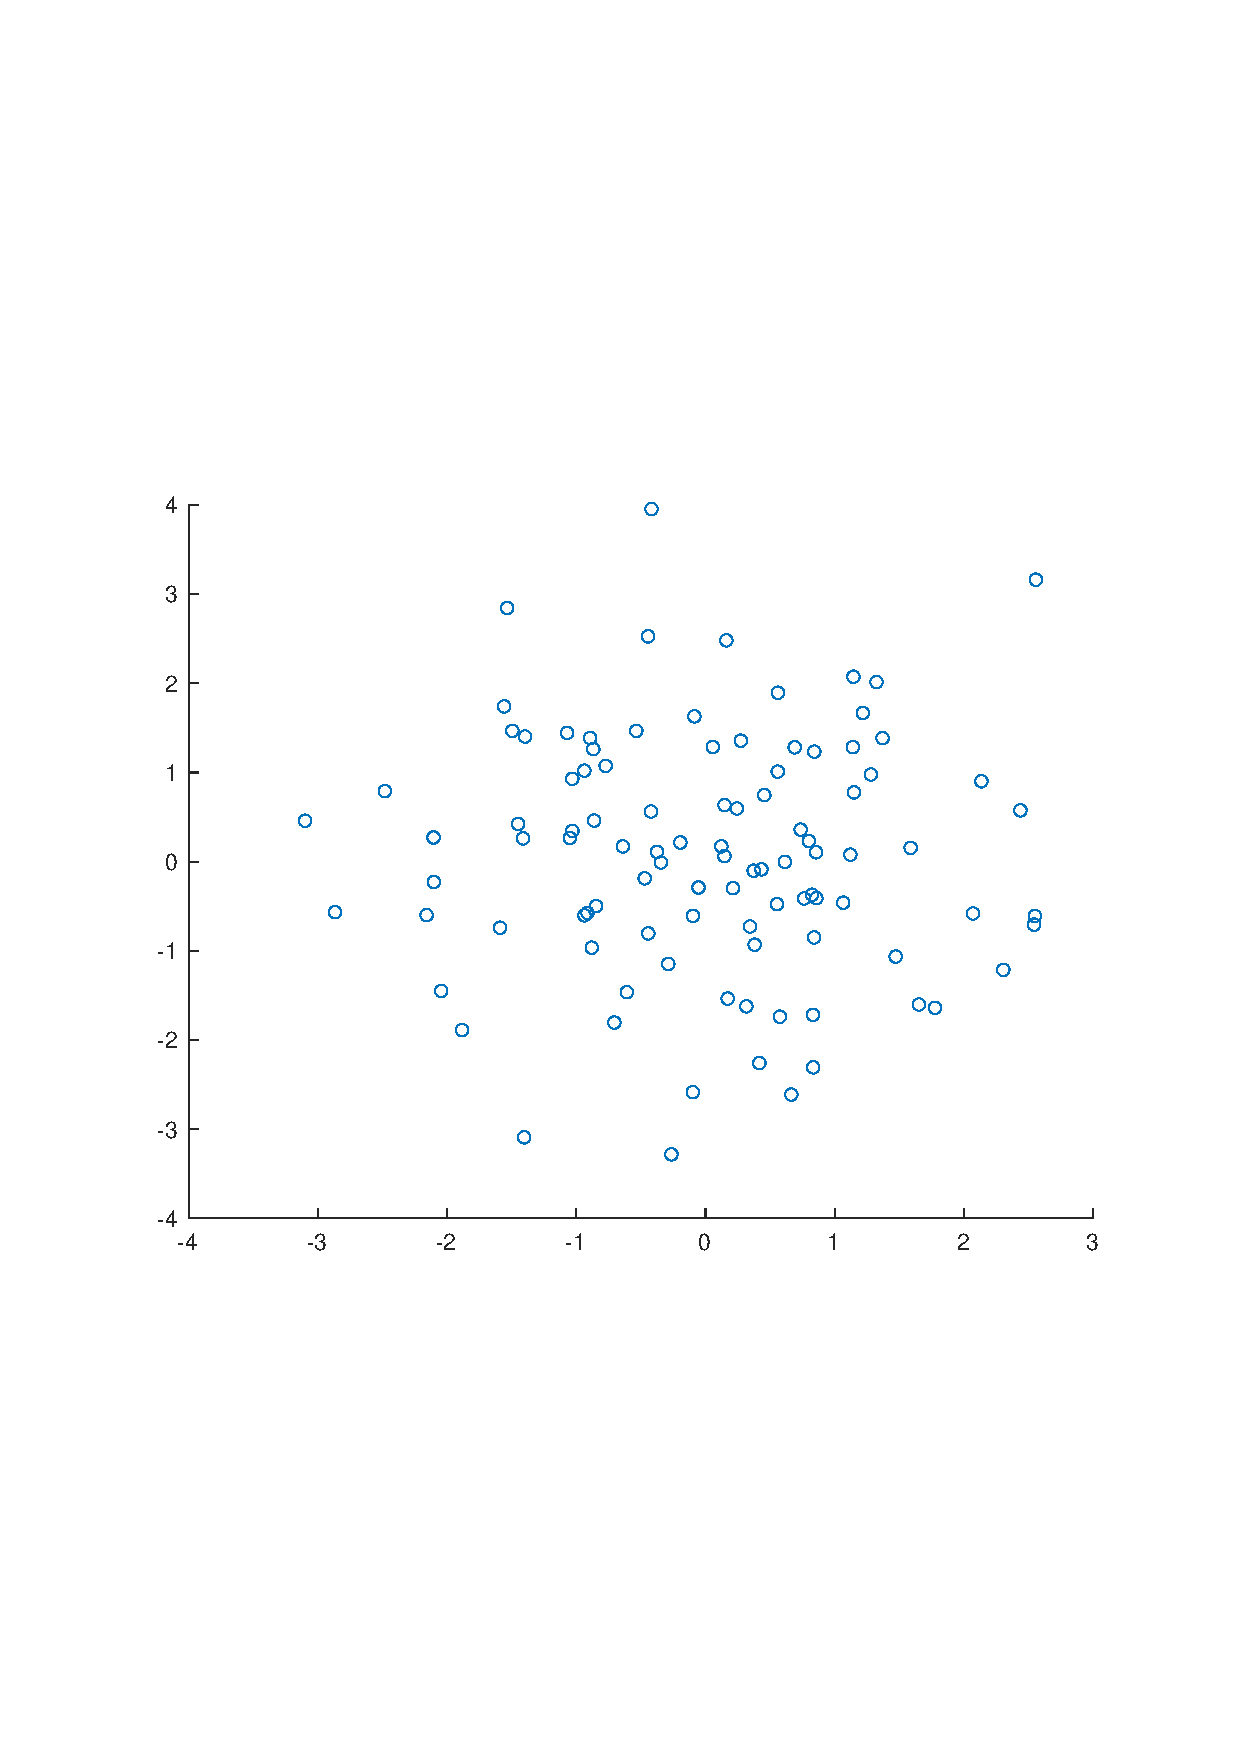
\includegraphics[width=0.4\textwidth]{83.pdf}  
	   		\captionsetup{labelformat=empty}\caption{3}
		\end{figure}
	\end{soln}
\item Make a scatter plot with a changed covariance matrix of $\begin{pmatrix}
    2 & 0.2 \\ 0.2 & 2\\
  \end{pmatrix}$.\\
  	\begin{soln}
  	    \begin{figure}[h!]
	        		\centering
	   		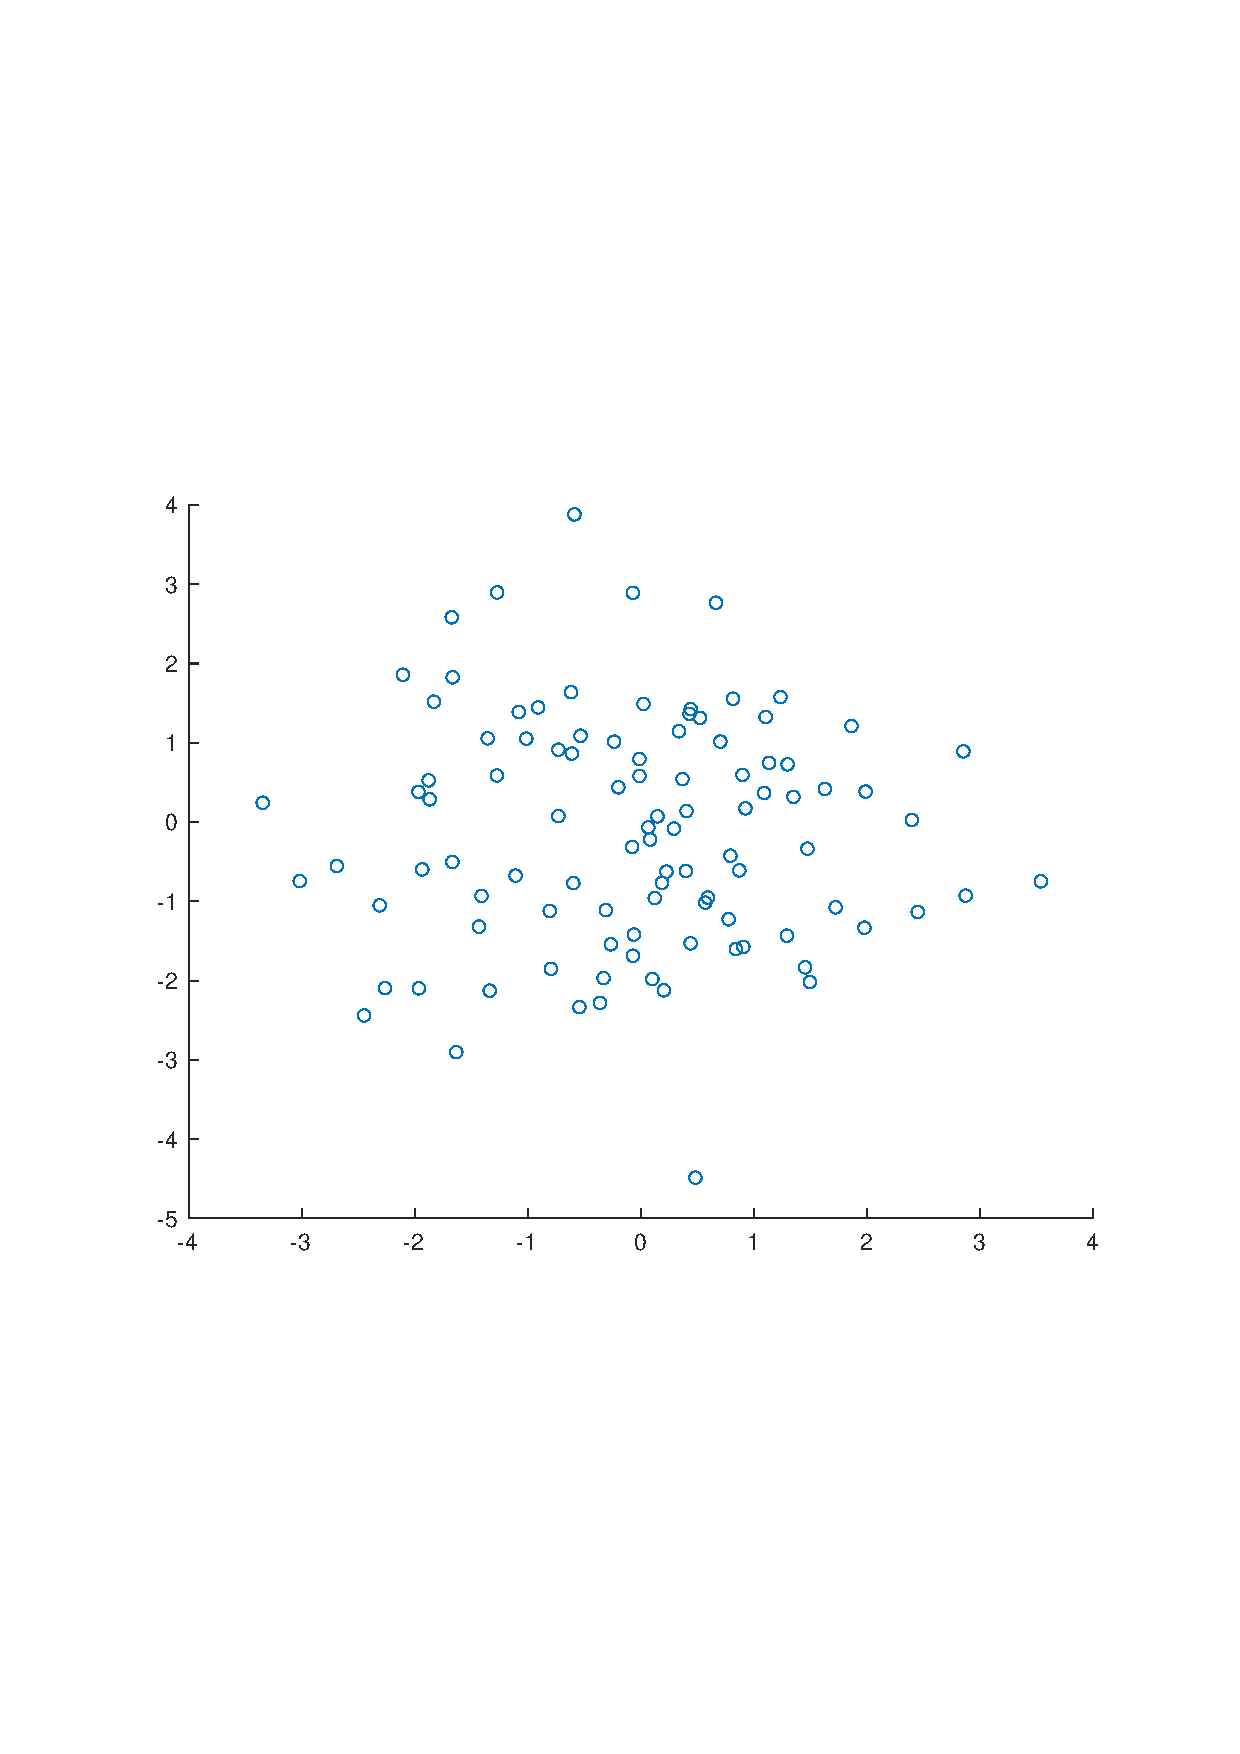
\includegraphics[width=0.4\textwidth]{84.pdf}  
	   		\captionsetup{labelformat=empty}\caption{4}
		\end{figure}

	\end{soln}
\item Make a scatter plot with a changed covariance matrix of $\begin{pmatrix}
    2 & -0.2 \\ -0.2 & 2\\
  \end{pmatrix}$.	\\
  	\begin{soln}
  	    \begin{figure}[h!]
	        		\centering
	   		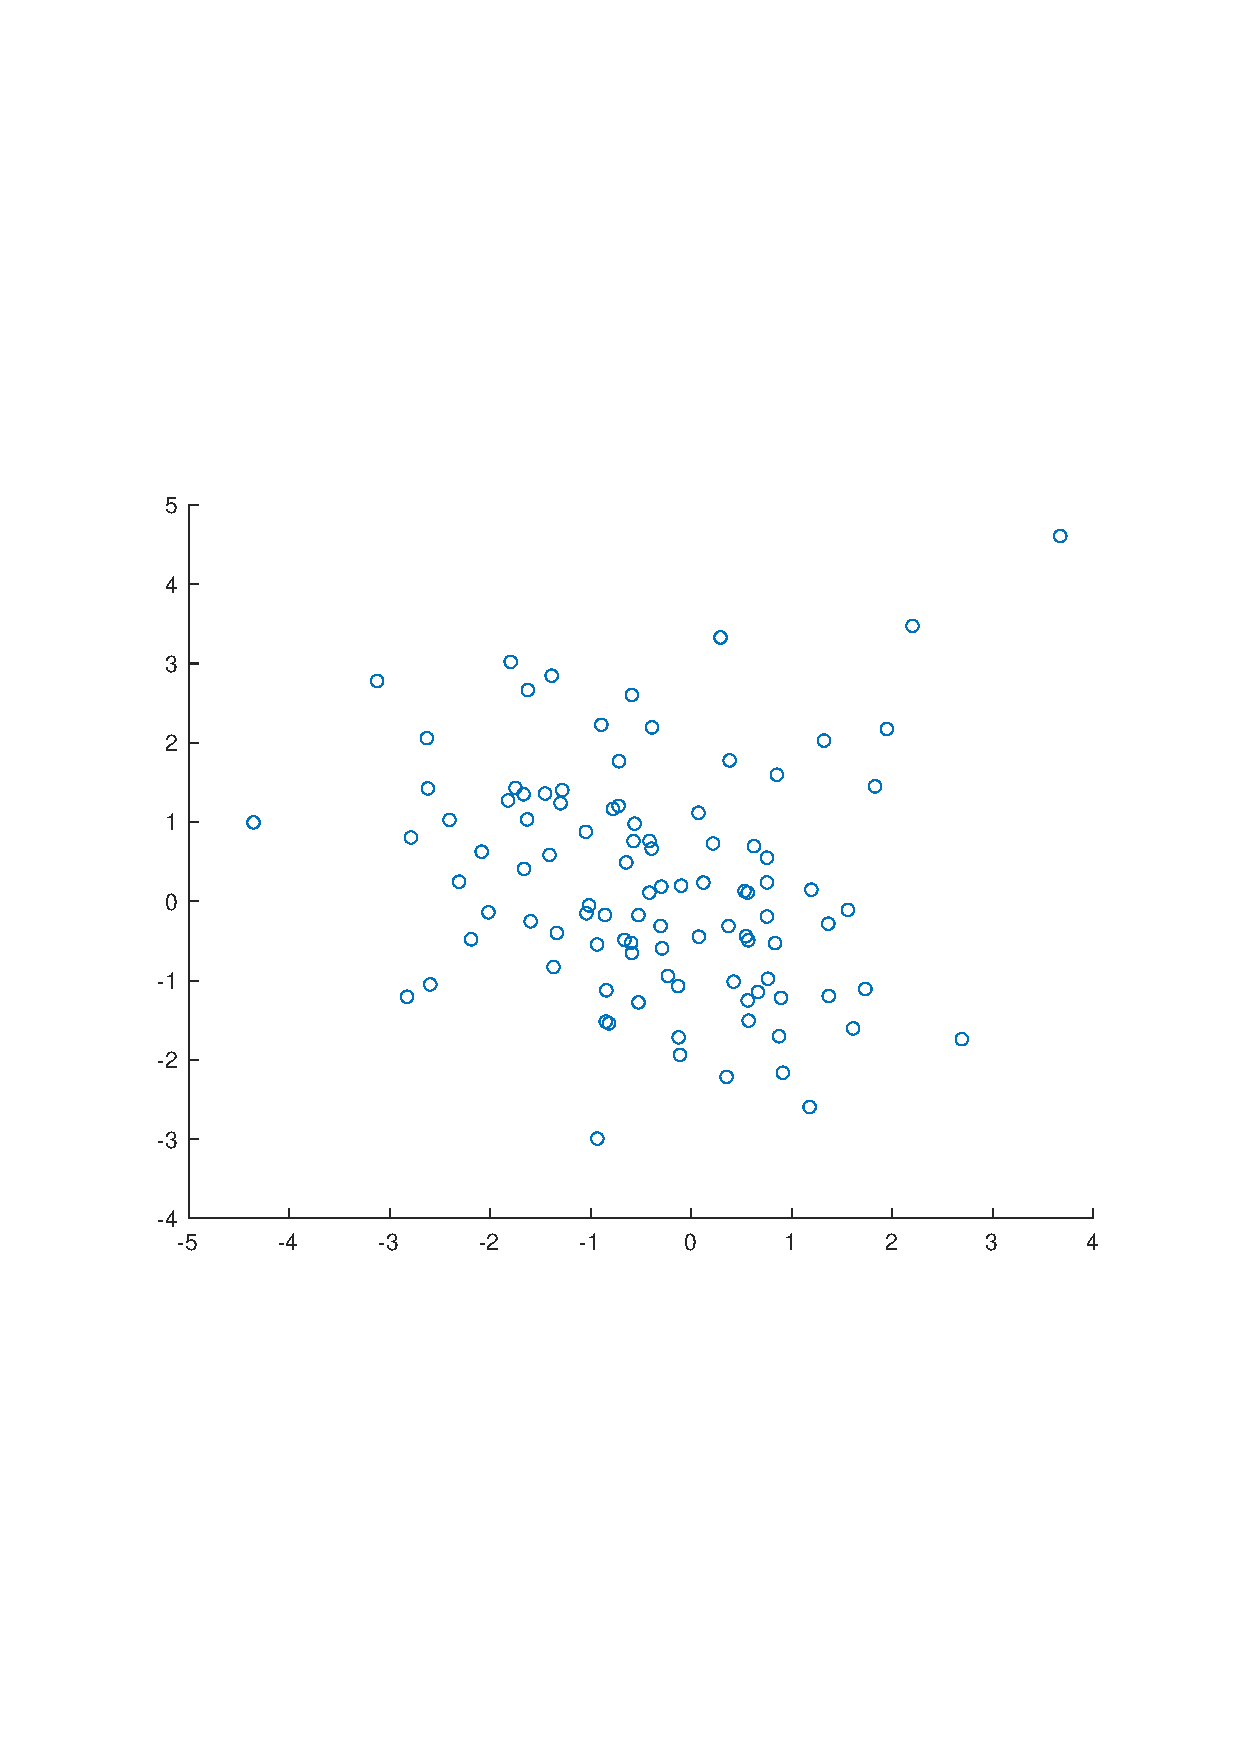
\includegraphics[width=0.4\textwidth]{85.pdf}  
	   		\captionsetup{labelformat=empty}\caption{5}
		\end{figure}

	\end{soln}
\end{enumerate}


\bibliographystyle{apalike}


%----------------------------------------------------------------------------------------


\end{document}
